\documentclass[border = 0.2cm]{standalone}
\usepackage{tikz}
\usepackage{amsmath,amssymb}

\usepackage[clock]{ifsym}
\usetikzlibrary{positioning,petri,arrows.meta, matrix}
\usetikzlibrary{patterns,decorations.pathreplacing}

\usepackage{pifont}
\usetikzlibrary{calc}
\newcommand{\vmark}{\ding{51}}
\newcommand{\xmark}{\ding{55}}
 
\begin{document}

\newcommand{\drawMonoflopFull}[7]{ 
\begin{scope}[#1]
    \node[place,tokens=#3, label=below left:off] (off) {};
    \node[place,tokens=#2, above=2.5cm of off, label=below left:enabled] (enabled) {};
    \node[transition, dashed, above left=1.25cm and 1.25cm of enabled, label={[align=center]below:fire!}] (trigger) {};
    \node[place,tokens=#4, right=2.5cm of off, label=below right:on] (on) {};
    \node[transition, above right=1.25cm and 1.25cm of off, label={[align=center]below:start!\\$p$\\$\langle 0 \rangle$}] (start) {#5};
    \node[transition, below right=1.25cm and 1.25cm of off, label={[align=center]below:stop!\\$\langle \delta \rangle$}] (stop) {#7};
    \node[transition, above=2.5cm of start, label={[align=center]below:fail!\\$1-p$\\$\langle 0 \rangle$}] (fail) {#6};
    
    \draw[bend left=30] 
        (trigger) edge[post, dashed] (enabled)
        (start) edge[pre] (enabled)
        (enabled) edge[post] (fail)
        (off) edge[post] (start) 
        (start) edge[post] (on) 
        (on) edge[post] (stop) 
        (stop) edge[post] (off); 
\end{scope}
}


\newcommand{\drawMonoflopSmall}[7]{ 
\begin{scope}[#1,
    on grid,
    node distance= 1cm,
    every place/.style={
        align=center,
        minimum width=2.5mm,
        minimum height=2.5mm
    },
    every transition/.style={
        font=\tiny,
        inner sep=0.5mm,
        align=center,
        minimum width=2.5mm,
        minimum height=2.5mm
    }]
    \node[place,tokens=#3] (off) {};
    \node[place,tokens=#2, above=of off] (trigger) {};
    \coordinate[left= 7.5mm of trigger] (input);
    \node[place,tokens=#4, right=of off] (on) {};
    \node[transition, above right=0.5cm and 0.5cm of off] (start) {#5};
    \node[transition, below right=0.5cm and 0.5cm of off] (stop) {#7};
    \node[transition, above=of start] (fail) {#6};
    
    \draw[dashed] (input) edge[post] (trigger);
    \draw[bend left=30] 
        (start) edge[pre] (trigger)
        (trigger) edge[post] (fail)
        (off) edge[post] (start) 
        (start) edge[post] (on) 
        (on) edge[post] (stop) 
        (stop) edge[post] (off); 
\end{scope}
}

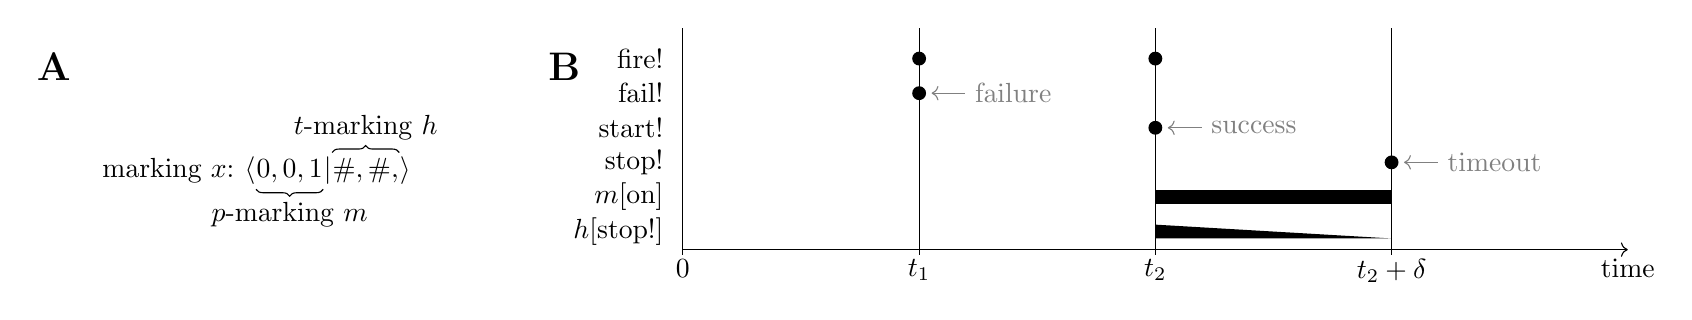
\begin{tikzpicture}[
    on grid,
    node distance= 1.5cm,
    every transition/.style={
        inner sep=1mm,
        align=center,
        minimum width=5mm,
        minimum height=5mm
    },
    dot/.style = {circle, fill, minimum size=5pt,
                  inner sep=0pt, outer sep=0pt},
    ]

\begin{scope}[local bounding box=A]
    % Draw petri net
    \drawMonoflopFull{}{0}{0}{1}{}{}{\Interval};

    % Add marking
    \path 
        node[anchor=base west, inner sep=0](state2) at (1cm,-4cm) {$|$} 
        node[left=0cm of state2.base west, anchor=base east, inner sep=0](state1){$0,0,1$} 
        node[label=left:{marking $x$:}, left=0cm of state1.base west, anchor=base east, inner sep=0] (state0){$\langle$}
        node[right=0cm of state2.base east, anchor=base west, inner sep=0](state3){$\#,\#,${\tiny\Interval}}
        node[right=0cm of state3.base east, anchor=base west, inner sep=0](state4){$\rangle$};
    
        \draw[decoration={brace, mirror, raise=2pt}, decorate] (state1.south west) -- (state1.south east) node[midway, below=3pt]{$p$-marking $m$};
        \draw[decoration={brace, raise=2pt}, decorate] (state3.north west) -- (state3.north east) node[midway, above=3pt]{$t$-marking $h$};
\end{scope}

\begin{scope}[local bounding box=B, shift={($(A.east)+(3cm,-1cm)$)}]
    % arrange coordinates
    \path coordinate[label=below:$0$](t0) coordinate[right=of t0](c1) coordinate[right=of c1, label=below:$t_1$](t1) coordinate[right=of t1](c2) coordinate[right=of c2, label=below:$t_2$](t2) coordinate[right=of t2](c3) coordinate[right=of c3, label=below:$t_2+\delta$](t3) coordinate[right=of t3](c4) coordinate[right=of c4, label=below:time](t4);
    
    % draw timeline
    \draw[->] (t0) -- (t4);
    \foreach \x in {t0,t1,t2,t3} 
        \draw ($(\x)+(0pt,8em)$) --  ($(\x)+(0pt,-2pt)$);
    
    % draw clock
    \node[above=3pt of t0, label=left:{$h[\text{stop!}]$}] (clkL) {};
    \path (clkL -| t2) coordinate(tmp1) -| coordinate(tmp2) (t3) ; 
    \fill[black] ($(tmp1)+(0pt,-2.5pt)$)-- ++(0pt,5pt)  -- ($(tmp2)+(0pt,-2.5pt)$) -- cycle;

    % draw EPSP
    \node[above=1.25em of clkL, label=left:{$m[\text{on}]$}] (pspL) {};
    \path (pspL -| t2) coordinate(tmp3) -| coordinate(tmp4) (t3) ; 
    \draw[line width=5pt] (tmp3) -- (tmp4);

    % draw stop
    \node[above=1.25em of pspL, label=left:{stop!}] (stopL) {};
    \path (stopL -| t3) node[dot](s1){}; 
    \draw[<-, bend left=30, gray] (s1.east) +(2pt,0mm) -- ++(5mm,0mm) node[anchor=west]{timeout};
   
    % draw start
    \node[above=1.25em of stopL, label=left:{start!}] (startL) {};
    \path (startL -| t2) node[dot](s2){}; 
    \draw[<-, bend left=30, gray] (s2.east) +(2pt,0mm) -- ++(5mm,0mm) node[anchor=west]{success};
    
    % draw fail
    \node[above=1.25em of startL, label=left:{fail!}] (failL) {};
    \path (failL -| t1) node[dot](s1){}; 
    \draw[<-, bend left=30, gray] (s1.east) +(2pt,0mm) -- ++(5mm,0mm) node[anchor=west]{failure};

    % draw inputs
    \node[above=1.25em of failL, label=left:{fire!}] (inpL) {};
    \path (inpL -| t1) node[dot](s1){} -| node[dot](s2){} (t2) ; 
    
    % draw transitions
    \foreach \x/\yOne/\yTwo/\yThree/\yFour/\yFive/\ySix in {t1/1/1/0/\xmark/\vmark/,t2/1/1/0/\vmark/\xmark/,t3/0/0/1///\vmark} 
        \drawMonoflopSmall{gray,every token/.style={fill=gray},shift={($(\x)+(-5mm,-2.5cm)$)}}{\yOne}{\yTwo}{\yThree}{\yFour}{\yFive}{\ySix};
    
    % draw states
    \foreach \x/\yOne/\yTwo/\yThree/\yFour/\yFive/\ySix in {c1/0/1/0///,c2/0/1/0///,c3/0/0/1///\Interval,c4/0/1/0///} 
        \drawMonoflopSmall{gray,every token/.style={fill=gray},shift={($(\x)+(-5mm,4cm)$)}}{\yOne}{\yTwo}{\yThree}{\yFour}{\yFive}{\ySix};
    
\end{scope}

% Add labels
\node at ($(A.north west)+(-5mm,5mm)$) (lA) {\Large \textbf{A}};
\node at (B.north west |- lA) {\Large \textbf{B}};

\end{tikzpicture}


\end{document}